\documentclass[12pt,a4paper, twoside]{report}
\usepackage[utf8]{inputenc}
\usepackage[english]{babel}
\usepackage{amsmath}
\usepackage{amsfonts}
\usepackage{amssymb}
\usepackage{graphicx}
\usepackage{lmodern}
\usepackage{tocbibind} % for toc, tof in table of contents
\usepackage{parskip}
\usepackage{url}
\usepackage[labelfont=bf]{caption} % for bold "figure 1.1"

% To have '-' instead of bullets in the itemize environment
\def\labelitemi{--}

% For hyperlinks and meta data
\usepackage{hyperref}
\hypersetup{
    bookmarks=true,         % show bookmarks bar?
    unicode=false,          % non-Latin characters in Acrobat’s bookmarks
    pdftoolbar=true,        % show Acrobat’s toolbar?
    pdfmenubar=true,        % show Acrobat’s menu?
    pdffitwindow=false,     % window fit to page when opened
    pdfstartview={FitH},    % fits the width of the page to the window
    pdftitle={Simulation of complex actuators},    % title
    pdfauthor={Hubert Woszczyk},     % author
    pdfsubject={Master thesis},   % subject of the document
    pdfcreator={TexMaker},   % creator of the document
    pdfproducer={ULg}, % producer of the document
    pdfkeywords={robotics, physics, bullet, blender, vrep, robocup}, % list of keywords
    pdfnewwindow=true,      % links in new PDF window
    colorlinks=true,       % false: boxed links; true: colored links
	linktocpage=true,    
    linkcolor=red,          % color of internal links (change box color with linkbordercolor)
    citecolor=blue,        % color of links to bibliography
    filecolor=magenta,      % color of file links
    urlcolor=cyan           % color of external links
}

% Margins
\usepackage[left=2cm,right=2cm,top=2cm,bottom=2cm]{geometry}

% For nice tables
\usepackage{booktabs,tabularx}
%\usepackage[tableposition=top]{caption}
%\captionsetup[table]{singlelinecheck=off}

\usepackage{cleveref} %should be the last package

\begin{document}

\begin{titlepage}


\begin{center}
\large
University of Liège - Faculty of engineering
\end{center}

\vfill

\begin{minipage}{0.5\textwidth}

\includegraphics[width=0.9\textwidth]{figures/ULg_logo_couleur.pdf}
\end{minipage}
\begin{minipage}{0.5\textwidth}
\huge
\textbf{Master thesis}\\\\
\normalsize
\textbf{Simulation of complex actuators}\\\\
Author : Hubert Woszczyk\\
Promotor : Pr. Bernard Boigelot\\
\end{minipage}

\vfill
\begin{center}
\large
Master thesis conducted for obtaining the\\ Master's degree in Electrical Engineering\\ by Hubert Woszczyk\\
\vspace*{8cm}
\normalsize
Academic year 2015-2016
\end{center}

\end{titlepage}

\newpage\null\thispagestyle{empty}\newpage

\thispagestyle{empty}
\begin{center}
    \Large
    \textbf{Simulation of complex actuators}
    
    \vspace{0.4cm}
    \large
    Hubert Woszczyk, under the supervision of Pr. Bernard Boigelot
    
    \normalsize
    Academic year 2015-2016\\
    Faculty of Applied Sciences\\
    Electrical Engineering
    
    \vspace{0.9cm}
    \textbf{Abstract}
\end{center}
The word \emph{robot} has been crafted by Czech writer Karel Čapek in his play R.U.R. (Rossum's Universal Robots) in the beginning of the XXth century and is derived from the slavic world \emph{robota} which means \emph{labour} or \emph{work}.


\clearpage
\pagenumbering{roman}
\setcounter{page}{1}
\chapter*{Acknowledgements}
My first thanks go to Prof. Bernard Boigelot who made it possible for numerous students, including me, to work in the passionate field of robotics. I also wish to thank him for his guidance, help and accessibility.

I am deeply grateful to my friends Elodie and Laurine for reading and correcting this manuscript. I also want to thank fellow students Grégory Di Carlo and Guillaume Lempereur with whom I had the pleasure of working together one last time.

Finally, I would like to express my sincere thanks to all those who helped me complete this master thesis.

\tableofcontents

\listoffigures

%% Intro
\clearpage
\setcounter{page}{1}
\pagenumbering{arabic}
\chapter{Introduction}
\section{Context}
For the last ten years, students from the Montefiore institute have been participating in a robotic contest named \emph{Eurobot}, a competition in which wheeled robots battle each other for points in various play environments. After some success and following a thirst for new challenges, it was decided to move on to another contest, \emph{RoboCup}.

\begin{figure}[htp]
\center
\begin{subfigure}[b]{0.45\textwidth}
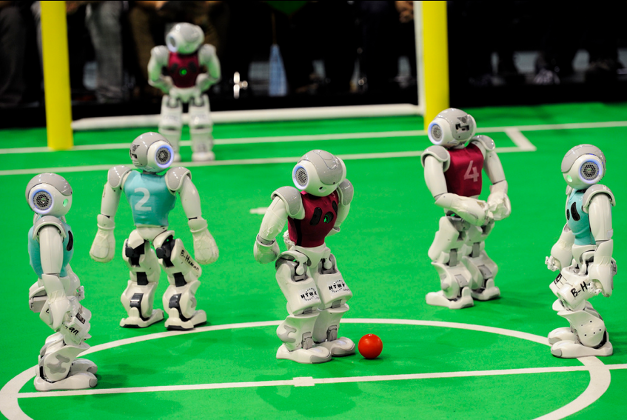
\includegraphics[width=\textwidth]{figures/intro_standard}
\caption[RoboCup Soccer standard platform]{Two teams of Nao robots playing against each other in the 2014 edition of RoboCup Soccer standard platform league. \textit{[Photo courtesy of RoboCup]}}
\label{fig:intro_standard}
\end{subfigure}
\hfill
\begin{subfigure}[b]{0.45\textwidth}
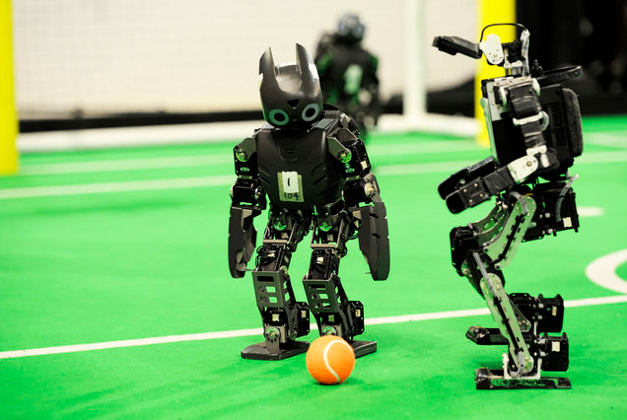
\includegraphics[width=\textwidth]{figures/intro_ks}
\caption[RoboCup Soccer standard platform]{Two robots of opposing teams looking at the ball, in the 2013 edition of RoboCup Soccer kidsize league. \textit{[Photo courtesy of RoboCup]}}
\label{fig:intro_ks}
\end{subfigure}
\caption[RoboCup standard and kidsize leagues]{Robocup standard and kidsize leagues}
\label{fig:intro_robocup}
\end{figure}

This contest is quite vast and, as of 2016, is divided into several categories (called domains in RoboCup jargon):
\begin{itemize}
\item RoboCup Rescue: as the name suggests, a domain where robots must perform various rescue operations in diverse scenarios.
\item RoboCup Industrial: a category with industrially oriented competitions.
\item RoboCup@Home: centred around domestic robots, such as robotics helpers for the elderly or robotic butlers.
\item RoboCupJunior: more of an initiative that aims to foster robotics interest in children rather than a contest, it helps organize various robotics events for younger minds.
\item RoboCup Soccer: historically the first category, centred about humanoid robots playing football. The objective of this category is to have a team of robots beat the world champions by 2050. This is the category we will compete in.
\end{itemize}

RoboCup Soccer is further subdivided into 4 sub-categories called leagues:\begin{itemize}
\item Standard platform, where the teams all use the same robot, \emph{Nao}, as illustrated in \Cref{fig:intro_standard}.
\item Simulation, a league that does not feature physical robots but focuses on team strategies and artificial intelligence. The matches take place in 2D or 3D simulators.
\item Adultsize, for the taller robots.
\item Teensize, for middle sized robots.
\item Kidsize, for the smaller robots. \Cref{fig:intro_ks} shows a match in progress from that league.
\end{itemize}

This year's team is preparing to participate to the Kidsize league and this master's thesis, along with two others, is the by-product of that team's activity. Since this is our first time participating we have no experience regarding humanoids robots. To avoid spending countless hours building and testing different designs we need a tool able of simulating a robot model and its interactions with a physical world.  

\section{Goals of the project}
The goal of this thesis is to provide the team with a physics simulating tool with the following features:
\begin{itemize}
\item realistic simulation of the physics of rigid bodies. This means that the tool should handle inertia, collisions, friction and constraints between objects. Simulation of springs and dampers is an interesting bonus.
\item receive and process orders incoming at a relatively high frequency. The processing need not be in real-time.
\item the model of our robot should receive the same orders as the real robot would. That is, the simulator should provide the same interface to the control code as the real robot would. 
\item 3D visualization of the simulation.
\end{itemize}

That simulator will be used to:
\begin{enumerate}
\item Test different robot designs and choose the best one, in a more efficient way than it could be achieved by physically building the designs.
\item Speed up development and testing of the control code because multiple teams will be able to work in parallel. 
\end{enumerate}

\section{Structure of the report}
This report begins with an overview of the basic concepts behind physics simulation on computers in \cref{chap:principles}. We then move on to \cref{chap:choice} that explains the problem we want to solve and motivates the choice of V-Rep as the main simulation tool for this project.

\Cref{chap:modelling} is about the modelling of our humanoid robot in preparation for \cref{chap:simulation} to go into the core of the subject with some simulations. \Cref{chap:simulation} also explains how our work influenced the design of the robot.

\Cref{chap:conclusion} concludes this work by summing up what is achieved and laying out future prospects.

%% Pre-work
\chapter{Choosing the tools}
In this chapter we discuss the choice of V-rep as the simulation tool for this project. We begin by explaining the basics of rigid body dynamics simulation, take a survey of some of the existing simulators and finally test some of them.

\section{Principles of rigid body dynamics simulation}
The section is heavily inspired by \cite{bender2014interactive}.
The basic idea behind the simulation of physics on a computer is to discretize time and apply the laws of newton to each object in the scene and integrate their acceleration during the timestep. When objects collide, collision.

A rigid body is an idealized solid object which will never change its shape, even under high forces.

The list of physics simulating engines is quite long, but the most popular ones are, in no particular order :
\begin{enumerate}
\item Bullet
\item ODE
\item DART
\item Simbody
\item PhysX
\item Havok
\end{enumerate}

\begin{table}[htp]
\center
\begin{tabularx}{\textwidth}{@{} X X X X X X @{}}
\toprule
\textbf{Engine} & \textbf{License} & \textbf{Coordinates} & \textbf{Origin} & \textbf{Editor} &\textbf{Solver type}\\ 
\midrule
Bullet & Free & Maximal & Games & Blender & Iterative \\ 

ODE & Free & Maximal & Simplified robot dynamics, games & & Iterative\\ 

DART & Free & Generalized & Computer graphics, robot control & &\\

Simbody & Free & Generalized & Biomechamics & \\

PhysX & Proprietary & Maximal & Games & \\

Havok & Proprietary & Maximal & Games & \\
\bottomrule
\end{tabularx}
\caption{Features comparison\cite{engines_comparison}}
\label{table:specs}
\end{table}

\section{Available simulators}
An integrated simulation tool is preferred over a bare-bones physics engine because :
\begin{itemize}
\item time would be lost on creating 3D visualization
\item time would be lost on writing code to import model
\item time would be lost on debugging
\end{itemize}
and all that before the actual work could begin.

\textbf{Blender\cite{Bruyninckx04}
} : \begin{itemize}
\item Uses the Bullet engine
\item Scripting via Python, remote control possible through socket
\item Very complete modelling tool, in a class of its own.
\item Comment : Hard to use because of obscure simulation options and difficulties to correctly set inertias
\end{itemize}

\textbf{Gazebo} : \begin{itemize}
\item Can use Bullet, Simbody, DART or ODE.
\item Scripting via C++
\item Uses SDF format for models.
\item Comment : Hard to use because model must be in SDF format, which no CAD excepted 3dworks exports to. Furthermore, compiled language takes longer to test.
\end{itemize}

\textbf{V-Rep}: \begin{itemize}
\item Can use Bullet, Newton or ODE.
\item Internal scripting in LUA, provides remote API class.
\item Can import 3D collada models.
\item Comment : Best tool so far because model can be imported and the inertias are easy to control, simulation options as well.
\end{itemize}

\textbf{Matlab}: \begin{itemize}
\item Analytical modelling
\item Mathcode
\item No visualization
\item Comment : Not adapted because tedious modelling and no visualization and hard to handle friction and difficult to handle other objects.
\end{itemize}

\begin{table}[htp]
\center
\begin{tabularx}{\textwidth}{@{} l l X X X X @{}}
\toprule
\textbf{Simulator} & \textbf{License} & \textbf{Physics engine(s)} & \textbf{Integrated editor} & \textbf{Modelling}\\ 
\midrule
Blender & Free & Bullet & Fully fledged & Internal\\ 

V-REP & Free (educational license) & Bullet, ODE, Newton, Vortex(10s limit) & Limited & Can import .COLLADA\\

Gazebo & Free & Bullet, ODE, Simbody, DART & Limited & SDF format\\

Webots & Proprietary & ODE & None & SDF format\\

Matlab & Proprietary & None & None & Mathematical\\
\bottomrule
\end{tabularx}
\caption{Comparison of simulators}
\label{table:simulators_comp}
\end{table}

\section{Choice}
Out of Gazebo, V-Rep and Blender, V-Rep is chosen as the best tool because\begin{itemize}
\item Gives the choice between 3 engines, something blender cannot do
\item Makes it easier than Gazebo to create models, because Gazebo uses the URDF format
\item Gives better access than blender to the physical options of the simulation (intertias, timestep of engine)
\item It is multi-platform. 
\end{itemize}

The physics engine used is Newton Dynamics because simple tests showed it to be the most stable with a high number of joints, with the exception of Vortex but it requires a license to run more than $10s$.

While Blender is not used as the primary simulation tool, it is used in the early phases of the modelling because it is what it does best. More on it in the next chapter. 

\chapter{Modelling tools usage}
This chapter covers the tools used in order to create a model of the robot, from the placement of the servos and joints to the incorporation of accelerometers.

\section{Blender}
The first stage of the modelling is done in Blender which is a lot more suited to this kind of work than V-Rep. 
Blender is used to do the following :
\begin{itemize}
\item place the servos, hinges and other elements in place.
\item simplify the servos, hinges into simple convex shapes with a low vertex count.
\item place position markers for the joints to be placed in V-Rep.
\end{itemize}

The model is finally exported in the COLLADA format.

\section{V-REP}
The model is finalized by :
\begin{itemize}
\item defining the mass and inertia of each piece(compiled in \cref{table:weights}) and enabling them for dynamic simulation.
\item adding joints between servos. For 2DOF joints, hinges are used as intermediates.
\item adding scripts to simulate sensors (COG, accelerometers).
\item adding springs on the legs through the use of prismatic and spheric joints.
\end{itemize}

\begin{table}[htp]
\center
\begin{tabularx}{\textwidth}{@{} X X X l @{}}
\toprule
\textbf{Module} & \textbf{Weight [$g$]} &  \textbf{Density [$g/m^3$]}& \textbf{Dimensions [$mm \times mm \times mm$]}\\ 
\midrule
Odroid C-2 & 40 &  & 85.0 x 56.0\\
Li-Po battery & 188 & 2000 & 103.0 x 33.0 x 34.0\\
Mx-28R & 72 & 1150 & 35.6 x 50.6 x 35.5\\
LI-USB30-M021C & 22 & 2200 & 26.0 x 26.0 x 14.7\\
Frame Fr-07 & & 1200 & \\
Frame Fr-101-H3 & 7 & 1200 & \\
\bottomrule
\end{tabularx}
\caption{Weights and dimensions of the pieces of the robot}
\label{table:weights}
\end{table}

\subsection{Servos}
Servos are simulated by joints.

\subsection{Joints}
Spherical joint : 3DOF angular.

Prismatic joint : 1DOF linear.

Revolute joint : 1DOF angular.

\subsection{Sensors (accel, cog)}
The COG is computed through a script inside V-Rep, attached to a piece of the model and made available through the remote interface\cite{vrep_manual}.



\subsection{Springs}
Springs are simulated by prismatic and spherical joints.

\chapter{Physical validation}
\section{Experimental set-up}
The set-up consists in :
\begin{itemize}
\item A camera that films the movements of a servo configuration.
\item A simulation of that servo configuration in V-Rep.
\end{itemize}

\begin{figure}[htp]
\center
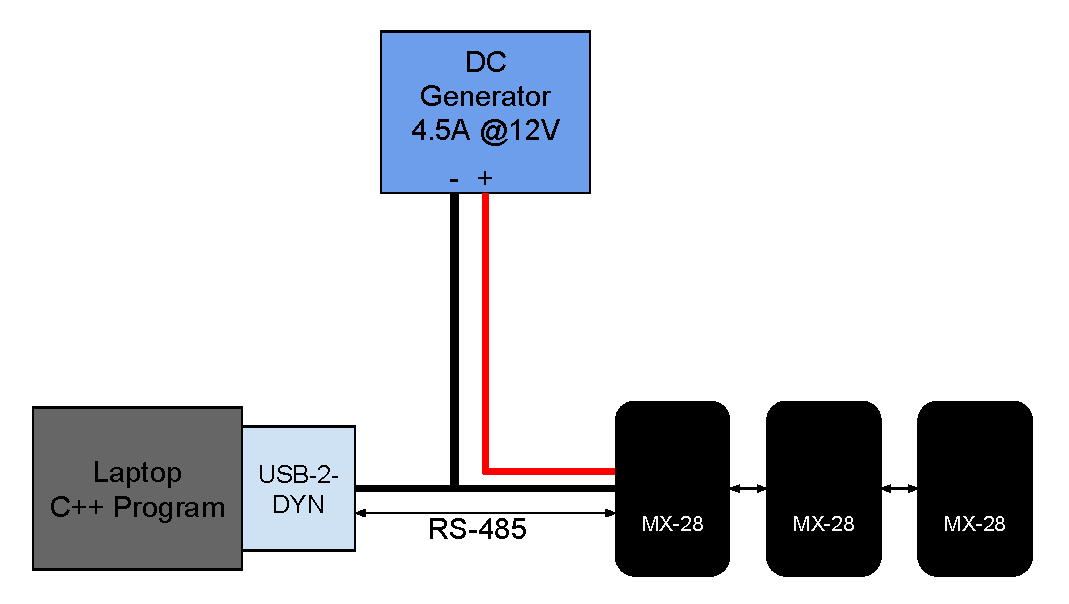
\includegraphics[width=0.6\textwidth]{figures/exp_setup}
\caption{Experimental setup}
\label{fig:exp_setup}
\end{figure}

\section{Experiments}
The first experiment is to test the torque : to that end, a frame is fixed onto a single servo and weighted. The setup is represented on \cref{fig:exp1}.

At $12V$, the maximal torque\cite{mx_28_manual} of the servo is supposedly $2.5N.m$. To test this, a weight of $2kg$ is hanged at $12.5cm$ from the center of the servo, because since 
\begin{align*}
2.5 - 9.81 \cdot (0.007 \cdot 0.01 + 0.016 \cdot 0.0725) &= x \cdot 0.125\\
x &= 20 N\\
&= 2.03 kg
\end{align*}

\begin{figure}[htp]
\center
    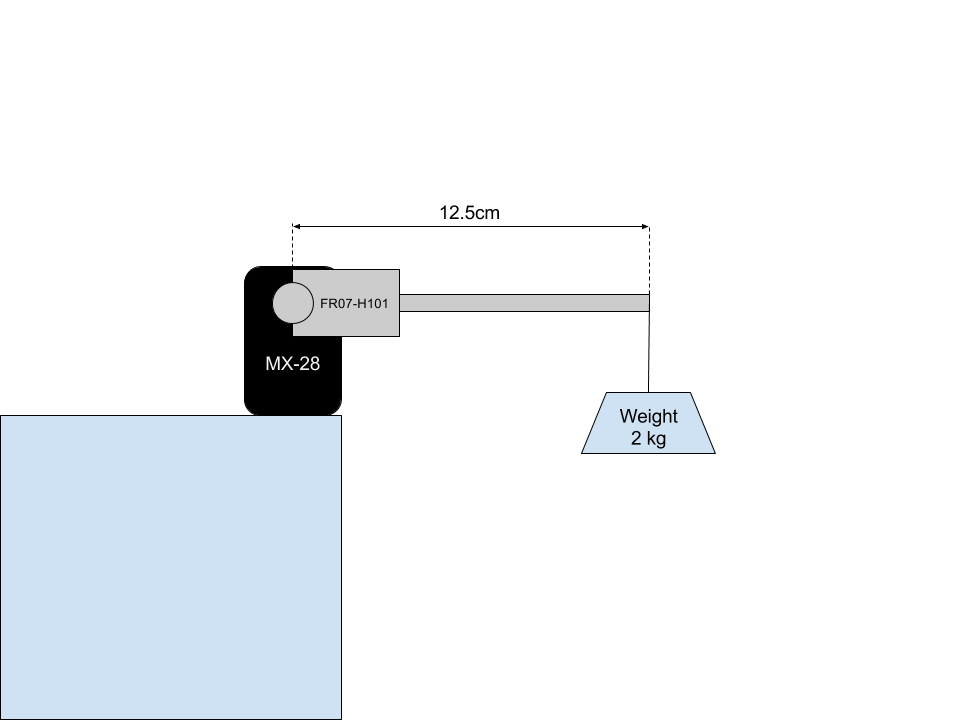
\includegraphics[width = 0.5\textwidth]{figures/exp1}
    \caption[Experimental setup for torque testing]{Experimental setup for torque testing : A weight of $2kg$ is suspended at $12.5cm$ from the servo, resulting in a torque of $2.5Nm$. The goal is to test whether the servo is able to move the weight upwards from the depicted initial situation.}
    \label{fig:exp1}
\end{figure}

Results
\begin{table}[htp]
\center
\begin{tabularx}{\textwidth}{@{}l X X X @{}}
\toprule
& \textbf{Stall torque @11.1V $[N.m]$} & \textbf{Stall torque @12V $[N.m]$} & \textbf{Stall torque @14.8V $[N.m]$}\\ 
\midrule
\textbf{Theoretical} & 2.1 & 2.5 & 3.1\\ 
\textbf{Experimental} &  &  & \\ 
\bottomrule
\end{tabularx}
\caption{Experimental stall torques at different tested voltages}
\label{table:exp1_results}
\end{table}

\section{Servo tuning}

\section{Results}

\chapter{Simulation}
In this section we will explain how to use the simulator and how it was used to influence the design of the robot. Finally some simulations will be shown.

\section{Simulation setup}
The basic idea of the simulation is presented on \cref{fig:simulation_principles}.

\begin{figure}[htp]
\center
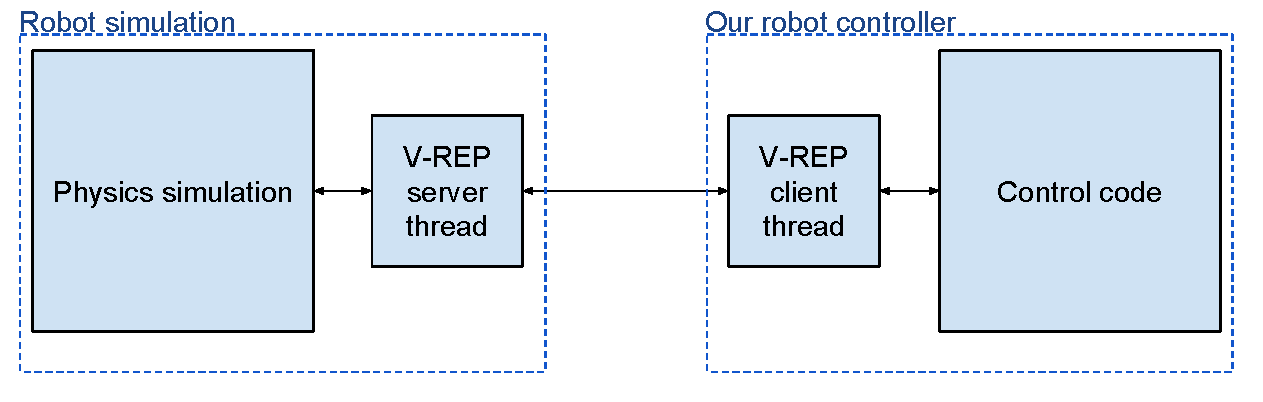
\includegraphics[width=0.6\textwidth]{figures/simulation_principles}
\caption[Simulation principles]{Simulation principles}
\label{fig:simulation_principles}
\end{figure}

The architecture of the system is explained on \cref{fig:remoteApi}. We choose to operate in the synchronous operating mode : before V-REP simulates a timestep it waits for a trigger, allowing us to precisely control the robot.

\begin{figure}[htp]
\center
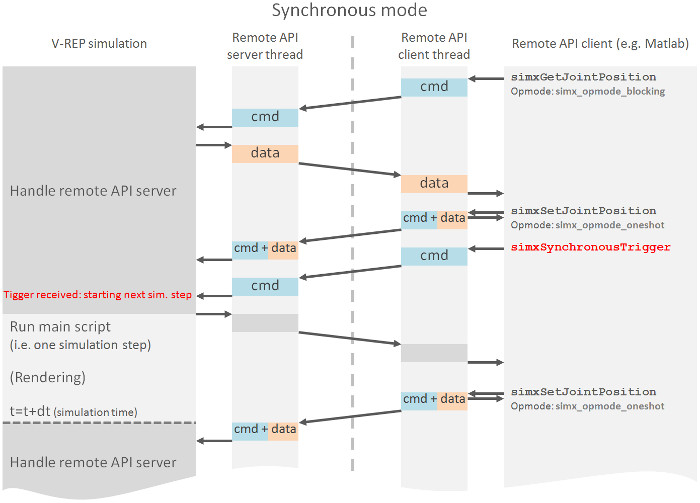
\includegraphics[width=0.6\textwidth]{figures/remoteApiSynchronous}
\caption[Simulation setup]{Explanation of the architecture of the simulation. The simulation runs on two threads : the simulation and the server thread. The server threads can receive orders from a client thread which is controlled by a custom application of our own.}
\label{fig:remoteApi}
\end{figure}

\section{Applications}
\subsection{Static stability}
The first application is simply to build a model of the robot and test if it is able to stand upright on its own. 

The different constituting elements are listed in \cref{table:weights}. 
\begin{table}[htp]
\center
\begin{tabularx}{\textwidth}{@{} X X X l @{}}
\toprule
\textbf{Module} & \textbf{Weight [$g$]} &  \textbf{Density [$kg/m^3$]}& \textbf{Dimensions [$mm \times mm \times mm$]}\\ 
\midrule
Odroid C-2 & 40 &  & 85.0 x 56.0 x 10.0\\
Li-Po battery & 188 & 2304 & 103.0 x 33.0 x 24.0\\
Mx-28R & 72 & 1150 & 35.6 x 50.6 x 35.5\\
LI-USB30-M021C & 22 & 2200 & 26.0 x 26.0 x 14.7\\
Frame Fr-07 & & 1200 & \\
Frame Fr-101-H3 & 7 & 1200 & \\
\bottomrule
\end{tabularx}
\caption[Weights and dimensions of the pieces of the robot]{Weights and dimensions of the pieces of the robot. The density is useful for the automatic computation of the weight and inertia of the pieces in V-REP.}
\label{table:weights}
\end{table}

The servos of the robot are simply ordered to hold their initial angle and the simulation determines that the robot can indeed stand upright without any active stabilization.

\subsection{Standing up routines}
This section is heavily inspired by \cite{Stuckler06}

\subsection{Walking}

\section{Influence on robot's design}
The simulator helped shape the robot through simulations that unveiled serious design problems (inability to stand after a fall, inability to walk).

The first design is visible on \cref{fig:first_robot}. It was plagued by stability problems, overcomplicated arms and simulation difficulties. 
\begin{figure}[htp]
\center
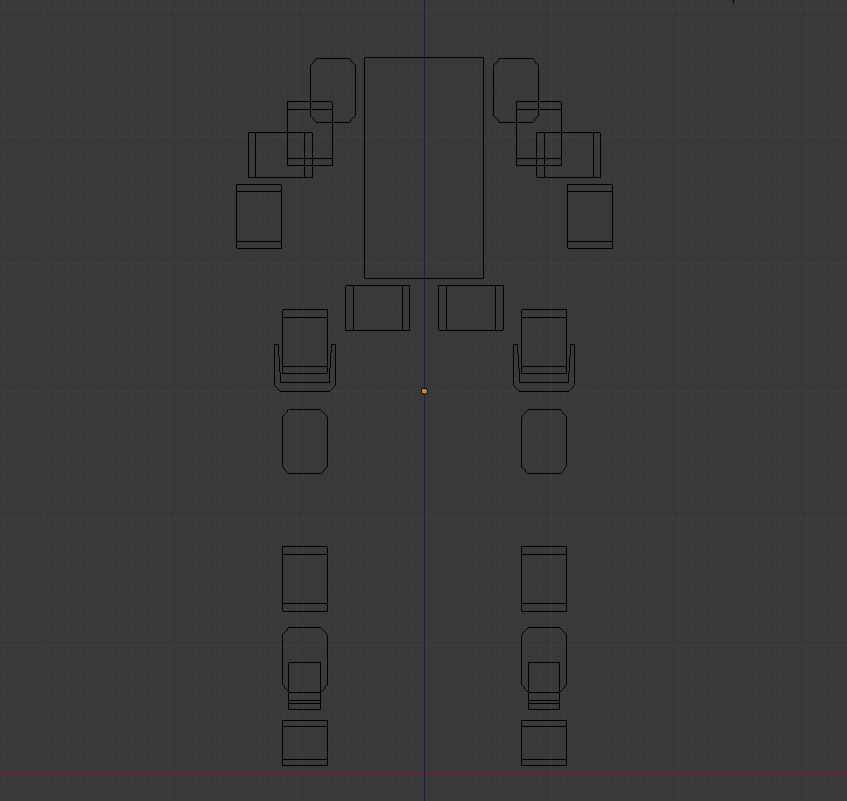
\includegraphics[width=0.6\textwidth]{figures/robot1}
\caption[Initial robot design]{First robot design. Arms use 4 servos each, making it quite heavy.}
\label{fig:first_robot}
\end{figure}

The final design, visible on \cref{fig:final_robot} has better stability, wider movement possibilities and can stand up and walk more easily. 
\begin{figure}[htp]
\center
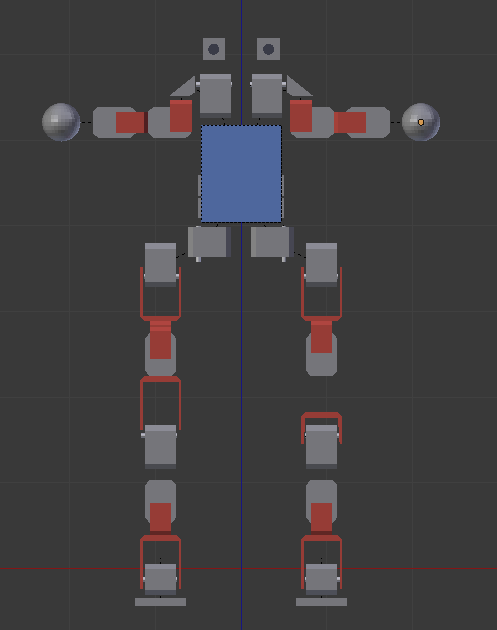
\includegraphics[width=0.6\textwidth]{figures/robot2}
\caption[Final robot design]{Final robot design. Arms now use 3 servos. The feet and the hips use a different configuration to have wider movement possibilities and bring down the center of gravity.}
\label{fig:final_robot}
\end{figure}

The final dimensions of the robot respect the rules of the contest:
\begin{itemize}
\item Height : $61.3cm$
\item Height of COM : $34cm$
\item Height of legs : $cm$
\item Height max is $< 1.5 \times 61.3$.
\item Foot area is $ cm^2$.
\end{itemize}

\chapter{Conclusion}
\section{Problems encountered}
A master thesis is a major endeavour and these are rarely devoid of obstacles. During this year several elements obstructed the completion of this work : \begin{itemize}
\item V-Rep is a fine tool but the lack of a proper internal modelling tool really hindered this work as every major modification meant that the whole model had to be modified in Blender and re-imported into V-Rep. This created a lot of overhead work which contributed nothing of interest to this work. 

This drawback is generalized amongst all the simulators that we surveyed at the beginning of this report and we feel it should be addressed quickly by their creators. Nevertheless, we understand that a modelling tool such as Blender took years to create so we would not expect simulators to catch up any time soon.

\item We also learned of the importance of studying mechanisms carefully before using them. Though things might appear simple at first, subtle implementation details might change everything. A fine example of that is us melting the core of the motor inside a MX-28R servo during our tests because of our trust in the announced safety mechanisms. Needless to say, they proved insufficient and we should have examined the documentation more closely.
\end{itemize}


\section{Future work}
\subsection{Modelling}
As of now it is still uncertain if Blender shall continue to support the COLLADA format (as explained in \cite{blender_roadmap}). In the negative, another tool should be chosen to perform the modelling.

The springs also need some work, as of now they are just there as a proof of concept but their parameters will need to be tuned.

As of now, the model uses simplified inertias, in the belief that a controller should be able to correct minor differences in behaviour between the model and the actual robot. In the case, theses inertias need to be more accurate, we suggest to use Meshlab\footnote{\url{http://meshlab.sourceforge.net/}} to compute the inertias of those objects.

\section{Conclusion}
This is the conclusion to my work.


\bibliographystyle{alpha}
\bibliography{bib}

\end{document}
